\documentclass[12pt]{article}
\usepackage[letterpaper, portrait, margin=1in]{geometry}
\usepackage{olesonaca}
\usepackage{lineno}
\usepackage[abbrvnat]{natbib}
\usepackage{setspace}
\usepackage{xcolor}
\usepackage{enumitem}
\usepackage{fancyhdr}
\pagestyle{fancyplain}
\usepackage[mmddyyyy]{datetime}
\renewcommand{\dateseparator}{.}
\renewcommand{\headrulewidth}{0pt}

\lhead{}
\rhead{}
\rfoot{}
\lfoot{}


\begin{document}

\noindent {\large \textsc{THERMOpy: A package for the reduction and analysis of U-Th-He Data.}} \\

\noindent Ethan Oleson

\doublespacing

\section{Introduction}
Thermochronology is a method that uses the interplay between the accumulation of radioactive daughter products from parent isotopes and the thermally activated diffusion of those daughter products from the crystal lattice \citep{zeitleretal1987, farleyetal1996, braunetal2006}. Exploiting this interplay allows one to constrain the timing of events with thermal signatures such as intrusion, exhumation, orogenesis, faults, and others \citep{braunetal2006}. Use of this method has only grown more popular since its reemergence in the late 1980s with \cite{zeitleretal1987}. Growth of this technique has stimulated new and exciting techniques, novel thermochronometers, and data analysis tools \citep{reinersetal2018, flowersetal2022a}. However, growth in the use of U-Th-He is not without pain.

With increased attention comes increased analysis approaches for the researcher to parse and determine what works for their study. Likewise, new methods of age calculation \citep{vermeesch2008} and error propagation \citep{martinetal2023}  cloud the field with differing interpretations all aimed at the same goal: producing the most accurate dates with highest certainty. Compounding this paradox of choice is the lack of standards for reporting and analytical practices. A recent series of publications, \cite{flowersetal2022a} and \cite{flowersetal2022b}, highlight that researchers and laboratories across the globe differ greatly on the amount of data reported, how the methods chosen are reported, and the method of analysis. The authors also highlight that no comprehensive data analysis tool exists. 

\subsection{Existing Software for Thermochronology Data Reduction and Analysis. }
Several programs exist for the reduction and analysis of thermochronologic data. These range from Excel plugins to R programs and Python scripts. Each one has its merits and shortcomings (summarized in the Table 2), yet all suffer from the same overall issues: 1) lack of choice and 2) no reporting infrastructure. Each existing package either requires the user to have ages and errors already calculated or it `forces' an approach on to the user with limited options for age calculations, error propagation, effective uranium calculation (eU), geometric parameters (ex. RS), etc. For example, \texttt{HeCalc} \citep{martinetal2023} allows the user to chose between either the iterative or non-iterative approximation of the production-diffusion equation from \cite{meestersanddunai2002a}, while \texttt{IsoplotR} \citep{vermeesch2018} does not report its age equation upfront, but only allows the use of one iterative solution, instead of pooled ages, geomteric ages, isochron ages, or a linear approximation function \citep{vermeesch2008}. Likewise, some software, such as \texttt{detritalPy} \citep{sharmanetal2018} is a primarily data visualization software and not a `one-stop shop'. While these packages exist, most labs still prefer Excel plugins due to the complexity and learning curve of the existing solutions. Although all of these software packages excel at certain functions and tasks, there is a lack of software that allows the user complete choice in approach, a workflow from raw data obtained from analysis to publication-quality figures, and ease of use. 

In this paper, I present a software that attempts to balance the call for better reporting with user-flexability as well as address the shortcomings of existing packages. 

\begin{table}[h!]
    \centering
    \begin{longtable}{p{3cm} p{3cm} p{5cm} p{4cm}}
        Program & Language or OS & Limitations & Reference \\ \hline
        Excel & Windows or Mac & different labs have different sheets, can’t handle large datasets, usually requires plotting to be done in illustrator or Inkscape. &&\\ 
        \texttt{HeCalc} & Python & limited in functions, choice, and requires proficiency in python. & \cite{martinetal2023} \\
        \texttt{detritalPy} & Python & Aimed towards detrital geochronology, for visualization. & \cite{sharmanetal2018} \\
        QTQt and HeFTy & Windows & powerful software for modeling, but lacks in initial interpretation options & \cite{gallagher2012, ketcham2005}, respectively. \\

        \texttt{IsoplotR} & R, online & Requires proficient knowledge of R, GUIs require manual entry of data. & \cite{vermeesch2018}
    \end{longtable}
       
  
    \caption{Existing software and packages for reducing, analyzing, and visualizing U-Th-He data with platform, limitations, and citation.}
    \label{tab:my_label}
\end{table}


\section{\texttt{THERMOpy} Overview}
\texttt{THERMOpy} is a package written in Python that is designed to reduce, analyze, and visualize thermochronologic data. It's main advantages are in flexibility; ease of use; breadth; broad use cases; and its open-source, OS-blind characteristics. It is designed so that anyone from a student with little to no experience in Python to a researcher famaliar with spreadsheet data reduction can utilize it. It's available features depend on the template data input format fed to the package. \texttt{THERMOpy} produces publication-quality plots and logs of the user's choice throughout the analysis session. A summary of the workflow for  \texttt{THERMOpy} can be found in Figure 1.

\subsection{Import Data}
Using the \texttt{dataimportsimple} function allows users to enter data that was reduced at another laboratory (see case study) and then quickly plot the data and obtain correlation values between age and other potential controls (effective uranium (eU), spherical radius (RS), maximum depositional age (MDA), and elevation). Users can also access more advanced functions (discussed below) by providing additional data. To access all functions, a user calls \texttt{dataimportfull} which takes a spreadsheet with sample information (name, location, etc.) grain information (geometric parameters and mineralogy), and raw concentrations of U, Th, He, and Sm. From these inputs, one can fully reduce their data by calculating grain characteristics (mass, surface area, volume, and spherical radius (RS)), raw ages from concentrations, effective uranium (eU), $F_T$ factor, and combine these calculations into a corrected age and other products. 

\subsection{Functions}
There are $\sim$ 30 functions that users can chose from to preform their desired analysis. These include geometric, mass, isotope, $F_T$ correction, eU, and age equations. There are several options for calculating these values from several publications. Although having multiple options for calculating your desired parameter may present a paradox of choice, it allows the user to decide what interpretation is best for their data. As with all choices in analysis, users are encouraged to report which equations they use. An example of where this choice is paramount is in defining the spherical radius of a grain for the $F_T$ alpha-ejection correction factor. It is common to calculate an RS by finding the raduis of sphere with the equivalent surface-area-to-volume ratio as your grain such that: $RS = (3V)/SA$, where $V$ is volume, and $SA$ is surface area \citep{farleyetal1996}. However, it has been shown to be more accurate to find the radius of the sphere with an equivalent $F_T$ factor: $ESR_{FT} = \overline{S}/(S/RS)$, where $\overline{S}$ is the mean weighted stopping distance and $S$ is the stopping distance of the isotope in the crystal  of interest \citep{cooperdocketal}. Depending on the equation in use, the resulting $F_T$ correction could be inaccurate \citep{ketchametal2011, cooperdocketal}.

The provided age functions present several methods of solving the same general equation: 
\begin{multline}
     ^4He = 8^{238}F_T^{238}U(e^{\lambda_{238}t} - 1) + 7^{235}F_T^{235}U(e^{\lambda_{235}t} - 1) \\  + 6^{232}F_T^{232}Th(e^{\lambda_{232}t} - 1) + ^{147}F_T^{147}Sm(e^{\lambda_{147}t} - 1) 
\end{multline}
Where $^{n}F_T^{n}$ are the isotope-specific $F_T$ correction, He, U, Th, and Sm are concentrations of the isotopes.  \citep{ketchametal2011}. There are several options for calculating age: \cite{meestersanddunai2002a} iterative and approximated age equation; linear age approximation \citep{vermeesch2008}; the pooled, central, and isochron age from \cite{vermeesch2008}; and an iterative solution the above $F_T$ corrected age \citep{ketchametal2011}. These choices allow the user maximum freedom to investigate how different age equations affect results. 

To perform the calculations in the software, $\sim 50$ parameters are defined including isotope stopping distances for apatite, zircon, titanite, monazite, xenotime, rutile, magnetite, hematite, goethite, and barite as well as decay constants for the $^{238}U$, $^{235}U$, $^{232}Th$ and $^{147}Sm$ chains \citep{ziegleretal2010, ketchametal2011}. 

\subsection{Error and Uncertainty}
In general, \texttt{THERMOpy} follows the form of other thermochronology software and takes an input, $A$, and used it to create a product, B, such that all functions take the form: $B = f(A)$. For almost all required quantities (ex. age) there is an associated error, $S(A)$ and thus $B$ has an error as well. \texttt{THERMOpy}, in its simplest usage shows error on all of its produced plots, in both the $x$ and $y$ directions. In it's `full' usage case, it preforms an error propagation and reports this data when it outputs. It contains functions for error and uncertainty from \cite{vermeesch2008}, \cite{reinersetal2018}, and \cite{martinetal2023}. 


\subsection{Products}
Several `products' come as standard. Plots of eU versus Age, RS versus Age, MDA versus Age (optional), and Elevation versus Age (optional) have dedicated functions.  These are called specifically, and can be saved (dpi = 300 by default) locally using a keyword argument: \texttt{save} in each function. The plots utilize \texttt{seaborn} functions and default to a simple design. Another plot that can be produced is a ``tectonic correlation diagram" which displays sample ID on the x-axis and corrected age on the x-axis. A blank column is plotted to furthest-right of the graph that allows space for the user to export the plot, import into a graphic design software (Illustrator, Inkscape, etc.), and annotate on the plot to display when certain tectonic events occurred compared to the sample age. The functionality to make this plot entirely within Python is a current area of development. All plots have the function to use default Adobe fonts provided the user has them installed locally. 

Both for simple and full analyses, two reports are produced: a results dataframe, and a parameter's table. Both of these reports are created and saved to the working directory upon calling a data import function. The results dataframe is initially populated with the data that you import and, as you perform your analysis, more columns are added such as: age and its error, $F_T$ correction, RS, etc. This dataframe is the main product of the analysis and can be adapted for publication. The parameters table is a .txt file that records the choices that the user makes. For instance, if the user chooses to use the eU calculation from \citep{shusteretal2006} versus the formula provided by \citep{cooperdocketal}, that choice will be recorded in the parameter table as: ``eU calc: Shuster et al., 2006". This table acts as a log of progress and history for the user, but also to encourage the reporting of the choices they make when the data is published. 
\begin{figure}[h!]
    \centering
    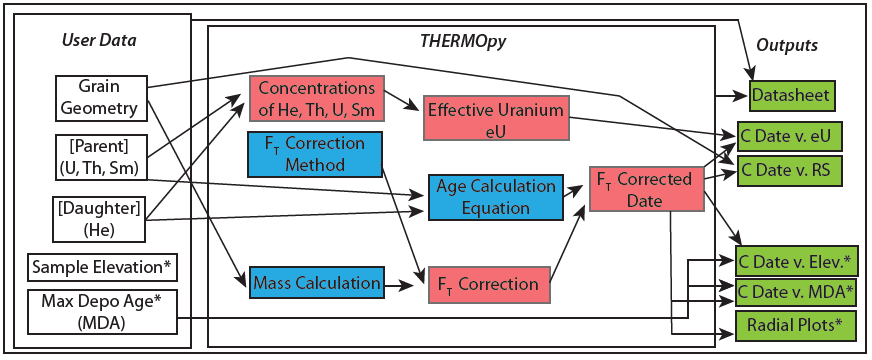
\includegraphics[scale=0.75]{proposal_figure_one.PNG}
    \caption{Flow chart of THERMOpy software. White blocks are user-entered data, blue are user choices, red is derived data, and green are THERMOpy products. An asterisk indicates optional data or products. Based on Figure 8 from Flowers et al. (2022).}
    \label{fig:enter-label}
\end{figure}

\section{Case Study: Great Valley forearc basin, California, USA. }

To elucidate the efficiency behind even the simple version of \texttt{THERMOpy}, plots of data from Oleson (2022) and Orme et al. (in prep) will be presented below. This data was collected from the Great Valley forearc basin, northern California, USA. The samples were coarse-grained sandstones from the basal units of the Great Valley Group (GVG) at the contact with the Coast Range Ophiolite (CRO) as well as blocks of serpentinite matrix melange \citep{oleson2022, Ormeetal2024}. The samples were taken to constrain the cooling rate of an intruded serpentinite diapir. Diapirs are mud volcanoes, and their emplacement within the GVG has been studied using fission track thermochronology \citep{vermeeschetal2006}. These samples were collected, processed with standard mineral separation techniques \citep{reinersetal2018}, packed, and analyzed using U-Th-He at the Arizona Noble Gas Laboratory at The University of Arizona. Data from the analysis was returned to the researchers already reduced using Excel. Since age, eU, RS, and associated errors were given by an outside lab, this case study utilizes the functions of THERMOpy simple - although \texttt{THERMOpy} could reconstruct from raw variables. 


To create the plots, data was imported using the \texttt{dataimportsimple()} function and was plotted using the \texttt{AgevRSdfsamp()}, \texttt{AgeveUdfsamp()}, \texttt{AgevMDAdfsamp()}, and \texttt{AgevElevdfsamp()}. These plotting functions only take a data frame as their argument. These functions visualize data in minutes and produce publication-ready plots. These four plots (Figure 2) represent 'standard' data visualization techniques for simple thermochronology studies. 
\begin{figure}
    \centering
    
\includegraphics[scale = 0.70]{oleson_2022_plots_with_legend_below.png.png}
    \caption{Plots of age versus eU, RS, MDA, and Elevation for samples from a serpentinite diapir in northern California. Notice the positive correlation between eU and age. All errors are $1\sigma$. Reproduced from \cite{oleson2022} using \texttt{THERMOpy}.} 
    \label{fig:enter-label}
\end{figure}

As the user produces these plots, they are presented with correlation statistics for the plotted quantities. For a thermochronology study, one does not want a correlation between age and eU or age and RS, as it could suggest that the source of the age is not some geologic event, like intrusion of a diapir. For instance, in Figure 2, there is an apparent positive correlation between eU and age. \texttt{THERMOpy} verifies this observation by indicating that age and eU have a Pearson's r-value of 0.54, with a p-value of 0.005. The software also tells you this is a moderate correlation and that the p-value is significant, based on our specified threshold (defaults to $\alpha = 0.05$). This r-value is not exceptionally high, however, using the plot of all the samples, we can see that 61121A may have a higher correlation factor. A plot of 61121A confirms this suspicion and returns an r-value of 0.99 and a p-value of 0.025. This quick analysis can allow the researcher to then investigate this relationship and find that positive date-eU correlations may be indicative of grains that have sustained radiation damage \citep{guenthneretal2013}. Grains with higher eU have sustained more damage, this leads to lower He diffusivity and an accumulation of He in the crystal \citep{guenthneretal2013, flowersetal2022a}. Alternatively, the sample has undergone slow, monotonic cooling - unlikely based on other ages from this dataset. These simple relationships can lead to important interpretations of thermochronologic data and it allows a user to make informed conclusions of their data after they confirm and understand the source of the statistics. 

\begin{figure}[h!]
    \centering
    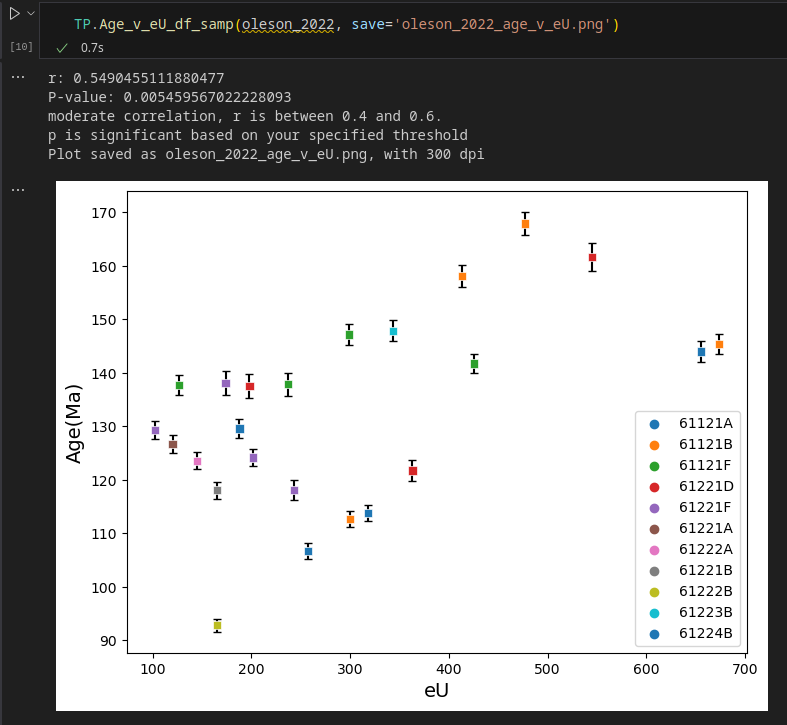
\includegraphics[scale = 0.75]{Age_v_eU.png}
    \caption{Screenshot of the view of the user when plotting Age versus eU for the northern California dataset. \texttt{THERMOpy} warns the user that there is a moderate correlation between Age and eU and that the p-value is significant based on the user defined threshold.}
    \label{fig:enter-label}
\end{figure}

\section{Conclusions}

In this paper, I have presented a software package for the reduction, analysis, and visualization of data in the (U-Th)/He system. This package is designed to give the user full flexibility in approach while also reporting choices made during the analysis session to encourage reporting in final publications. I have also shown that, the intuitive and simple functions of \texttt{THERMOpy} allow for the quick and easy interpretation of data for users spanning the spectrum of Python familiarity, and experience with data analysis. 
\newpage
\bibliographystyle{ewo_gsa_23}
\bibliography{thermomaster}
\end{document}
